\begin{frame}{Design Objectives}
	\begin{columns}[T]
		\begin{column}{0.5\textwidth}

			\begin{enumerate}

				\item \textbf{Omnidirectional movement}


				\item \textbf{Kicker}
				      % The robot needs to be able to move with the ball.

				\item \textbf{Dribbler}
				      % The design choices made when building the robot needs to be made in such way that the platform can evolve and improve in in future iterations of this project.

				\item \textbf{Real-time control}
				      % The robot needs to be able to pass and kick the ball.

				\item \textbf{Modularity}

			\end{enumerate}
		\end{column}
		\begin{column}{0.5\textwidth}
			\begin{adjustbox}{scale=2,center,margin={-1cm,3cm,2cm,0cm}}
				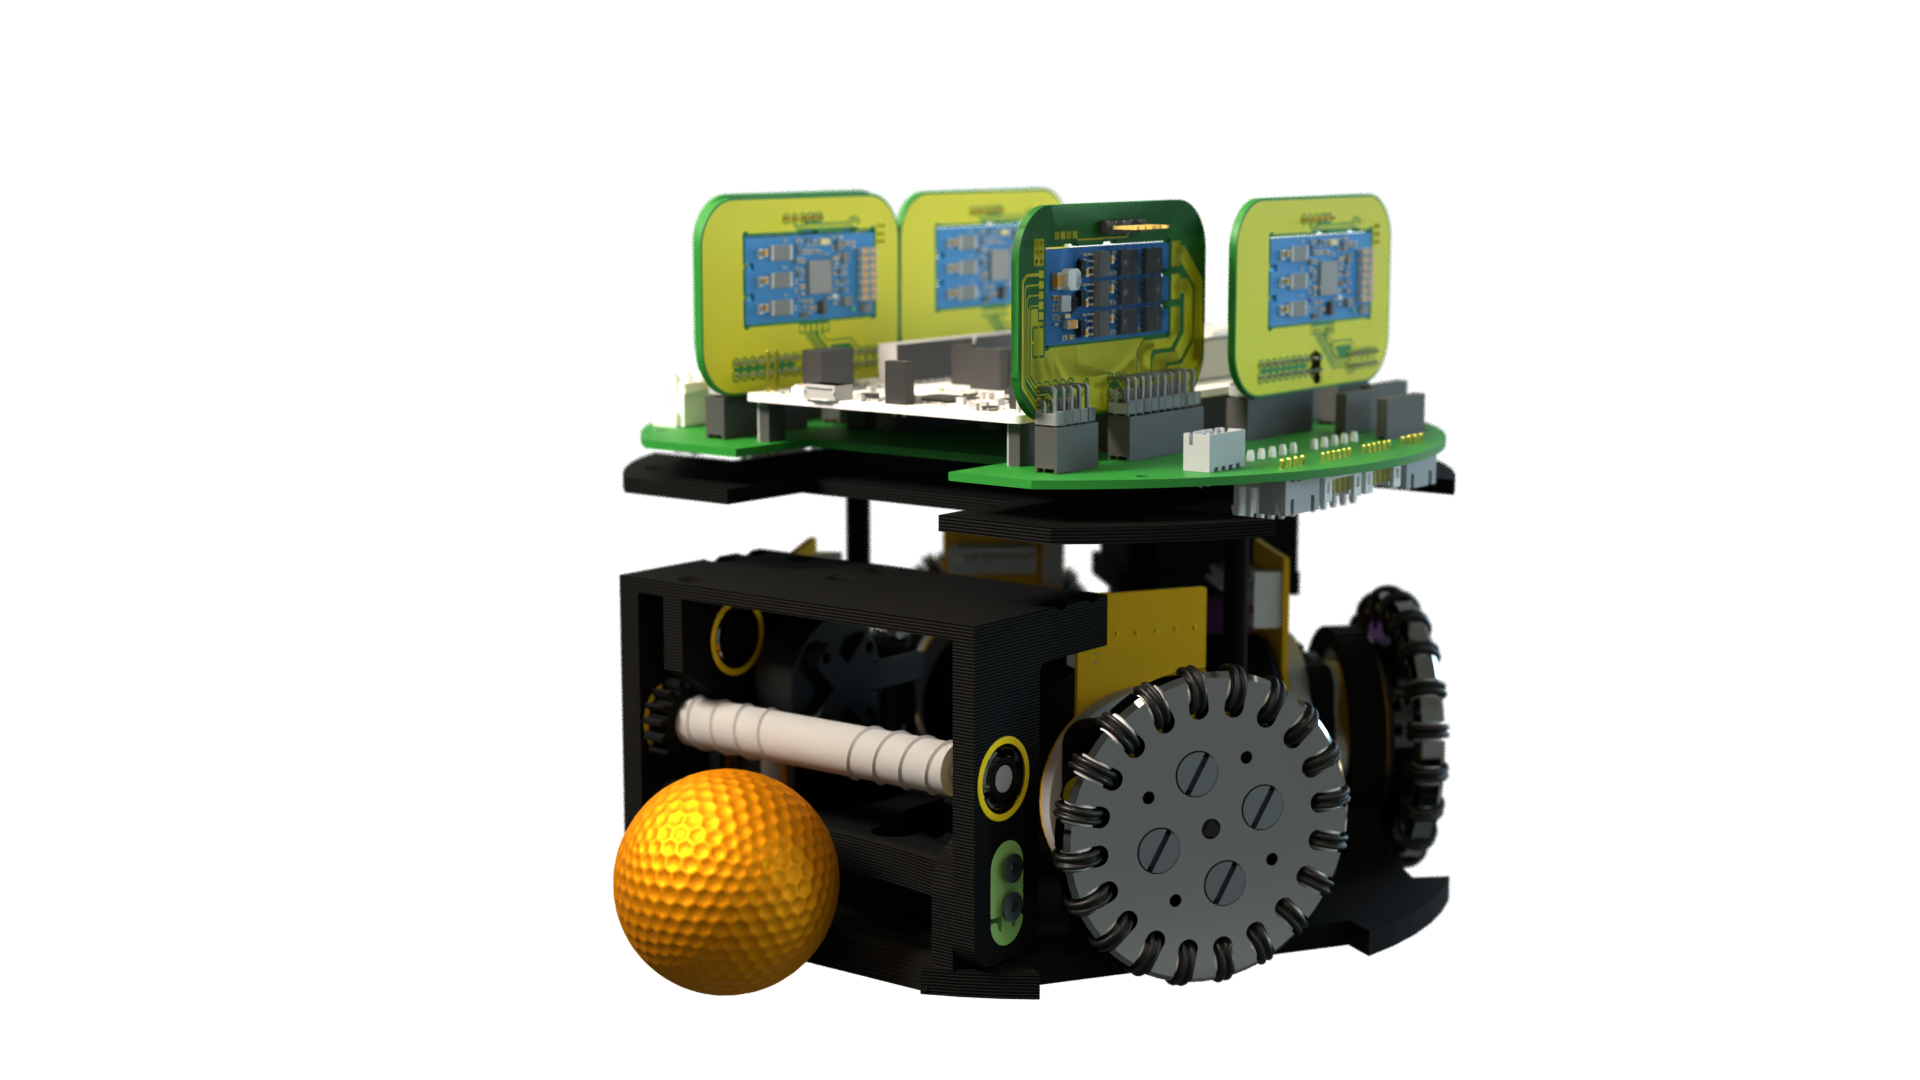
\includegraphics[width=\textwidth]{image/png/robot_base.png}
			\end{adjustbox}
		\end{column}
	\end{columns}
\end{frame}
